\documentclass[paper=a4, fontsize=11pt]{scrartcl} % KOMA-article class

%-------------------------------------------------
%   THEMES, PACKAGES, CUSTOM COMMANDS
%-------------------------------------------------
\usepackage{blindtext}
\usepackage[english]{babel}                             % English language/hyphenation
\usepackage[protrusion=true,expansion=true]{microtype}  % Better typography
\usepackage{amsmath,amsfonts,amsthm}                    % Math packages
\usepackage[pdftex]{graphicx}                           % Enable pdflatex
\usepackage[export]{adjustbox}
\usepackage[svgnames]{xcolor}                           % Enabling colors by their 'svgnames'
\usepackage[hang, small,labelfont=bf,up,textfont=it,up]{caption} % Custom captions under/above floats
\usepackage{subcaption}
\usepackage{epstopdf}       % Converts .eps to .pdf
%\usepackage{subfig}         % Subfigures
\usepackage{booktabs}       % Nicer tables
\usepackage{fix-cm}         % Custom fontsizes
\usepackage{listings}
\usepackage{soul}
\usepackage{float}

\usepackage{hyperref}

\usepackage[foot=30pt,margin=1in]{geometry}

% Custom sectioning (sectsty package)
\usepackage{sectsty}
\allsectionsfont{
    \usefont{OT1}{phv}{b}{n}    % bch-b-n: CharterBT-Bold font
}
\sectionfont{
    \usefont{OT1}{phv}{b}{n}
}

% Custom colors
\definecolor{brsugrey}{rgb}{0.9, 0.9, 0.9}
\definecolor{brsublue}{rgb}{0, 0.594, 0.949}

%
\newcommand{\upperRomannumeral}[1]{\uppercase\expandafter{\romannumeral#1}}

% Creating an initial of the very first character of the content
\usepackage{lettrine}
\newcommand{\initial}[1]{%
    \lettrine[lines=3,lhang=0.3,nindent=0em]{
        \color{brsublue}
        {\textsf{#1}}}{}}

%-------------------------------------------------
%   COMMON INFO
%-------------------------------------------------
\newcommand{\hmwkTitle}{Week \upperRomannumeral{4} report}
\newcommand{\hmwkDueDate}{Monday, October 17, 2016}
\newcommand{\hmwkClass}{Scientific Evaluation and Experimentation}
\newcommand{\hmwkClassShort}{SEE WS2016}
\newcommand{\hmwkAuthorFullName}{Minh H. Nguyen \& Bach D. Ha}
\newcommand{\hmwkAuthorLastName}{Nguyen \& Ha}
\newcommand{\hmwkAuthorEmail}{minh.nguyen@smail.inf.h-brs.de\\
                              bach.ha@smail.inf.h-brs.de}
\newcommand{\hmwkAuthorInstitute}{BRS University of Applied Sciences}

%-------------------------------------------------
%   HEADERS & FOOTERS
%-------------------------------------------------
\usepackage{fancyhdr}
\pagestyle{fancy}
\usepackage{lastpage}
% Header (empty)
\lhead{}
\chead{}
\rhead{}
% Footer (you may change this to your own needs)
\lfoot{\footnotesize
    \texttt{\hmwkClassShort} ~
    \textbullet ~ \hmwkAuthorLastName ~
    \textbullet ~ \hmwkTitle}
\cfoot{}
\rfoot{\footnotesize page \thepage\ of \pageref{LastPage}}  % "Page 1 of 2"
\renewcommand{\headrulewidth}{0.0pt}
\renewcommand{\footrulewidth}{0.4pt}

%-------------------------------------------------
%   TITLE & AUTHOR
%-------------------------------------------------
\usepackage{titling}

\newcommand{\HorRule}{\color{brsublue}% Creating a horizontal rule
    \rule{\linewidth}{1pt}%
    \color{black}
}

% Title
\pretitle{
    \vspace{-30pt}
    \begin{flushleft}
        \HorRule
        \fontsize{22}{22} \usefont{OT1}{phv}{b}{n} \color{gray} \selectfont
}
\title{\hmwkClass \\
       \hmwkTitle}
\posttitle{
    \par
    \end{flushleft}
    \vskip 0.5em
}

% Author
\preauthor{
    \begin{flushleft}
        \large \lineskip 0.25em
        \usefont{OT1}{phv}{b}{sl} \color{brsublue}}

\author{\hmwkAuthorFullName}

\postauthor{
        \footnotesize
        \usefont{OT1}{phv}{m}{sl} \color{Black}
        \\\hmwkAuthorInstitute
        \\\hmwkAuthorEmail
        \par
    \end{flushleft}
    \HorRule}

% Date
\date{\hmwkDueDate}

%-------------------------------------------------
%   BEGIN
%-------------------------------------------------
\begin{document}
    \maketitle
    \thispagestyle{fancy} % Enabling the custom headers/footers for the first page
    
    \section{Principal Component Analysis}

    \subsection{Going straight forward}
    \begin{figure}[H]
        \begin{center}
            \setlength{\fboxsep}{0.5pt} %
            \setlength{\fboxrule}{0.5pt}
            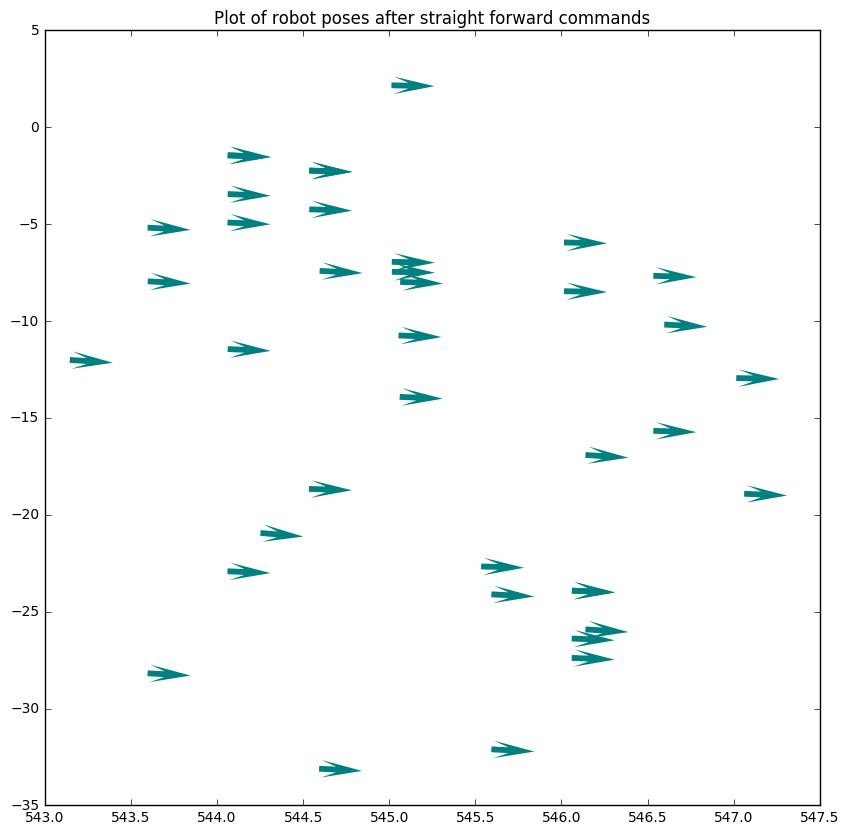
\includegraphics[width=0.7\linewidth,fbox]{images/poses_plot_1_straight.png}
            \caption{Recorded poses of the LeJOS robot going straight forward.}
        \end{center}
    \end{figure}
    \begin{figure}[h!]
        \begin{center}
            \setlength{\fboxsep}{0.5pt} %
            \setlength{\fboxrule}{0.5pt}
            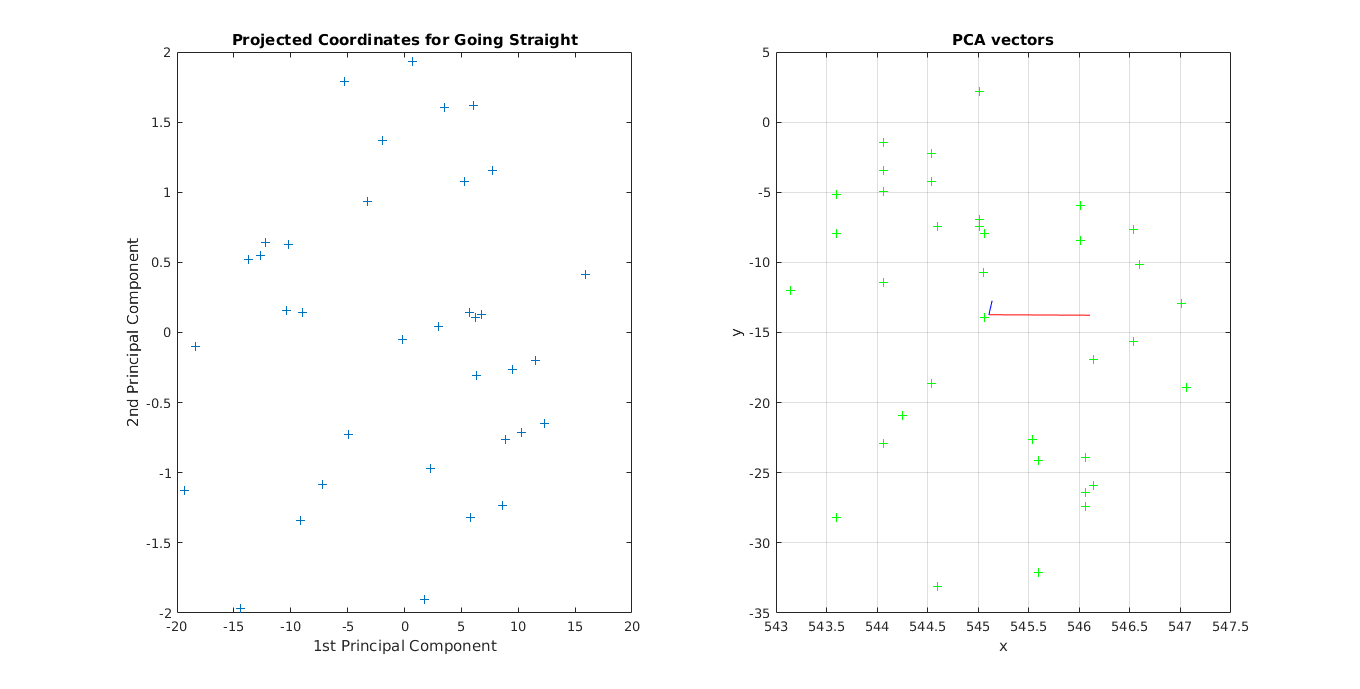
\includegraphics[width=\linewidth,fbox]{images/pca_straight.png}
            \caption{PCA analysis of straight forward movement.}
        \end{center}
    \end{figure}
    \begin{figure}[h!]
        \begin{center}
            \setlength{\fboxsep}{0.5pt} %
            \setlength{\fboxrule}{0.5pt}
            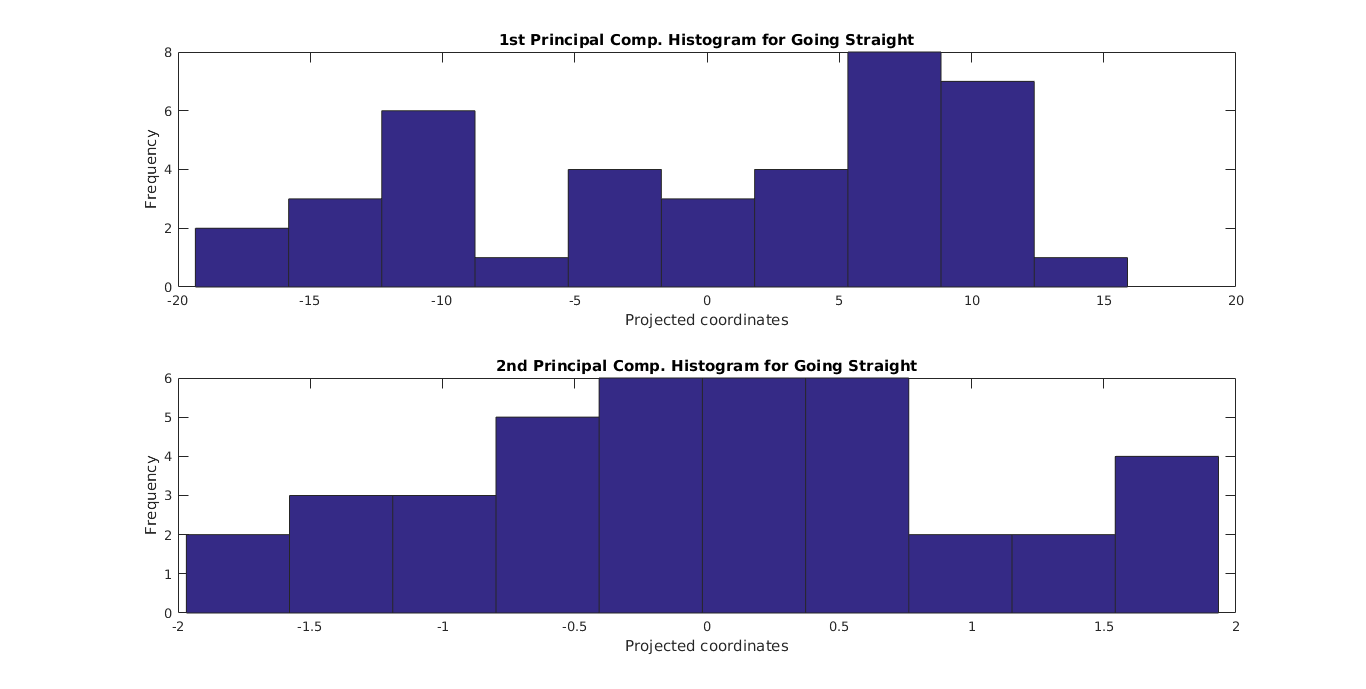
\includegraphics[width=\linewidth,fbox]{images/pca_histogram_straight.png}
            \caption{Histograms of coordinates projected onto principal components for straight forward movement.}
        \end{center}
    \end{figure}

    \subsection{Going slightly left}
    \begin{figure}[h!]
        \begin{center}
            \setlength{\fboxsep}{0.5pt} %
            \setlength{\fboxrule}{0.5pt}
            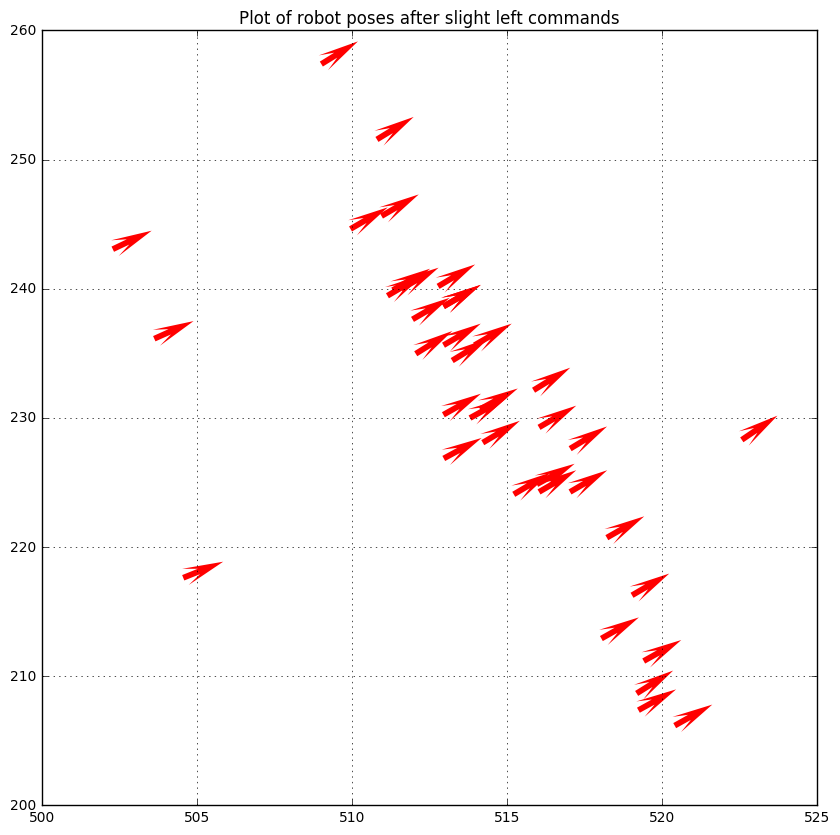
\includegraphics[width=0.7\linewidth,fbox]{images/poses_plot_2_slightLeft.png}
            \caption{Recorded poses of the LeJOS robot going slightly left.}
        \end{center}
    \end{figure}

    \begin{figure}[h!]
        \begin{center}
            \setlength{\fboxsep}{0.5pt} %
            \setlength{\fboxrule}{0.5pt}
            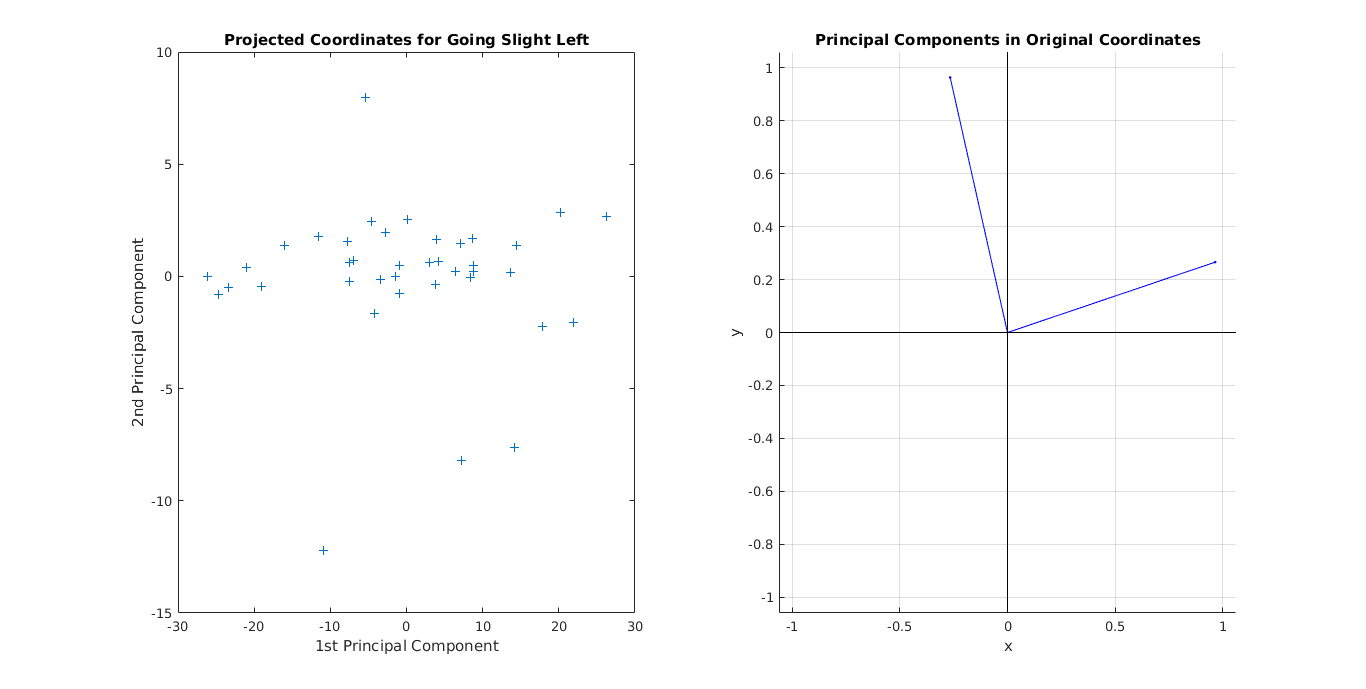
\includegraphics[width=\linewidth,fbox]{images/pca_slightLeft.png}
            \caption{PCA analysis of slight left movements.}
        \end{center}
    \end{figure}

    \begin{figure}[h!]
        \begin{center}
            \setlength{\fboxsep}{0.5pt} %
            \setlength{\fboxrule}{0.5pt}
            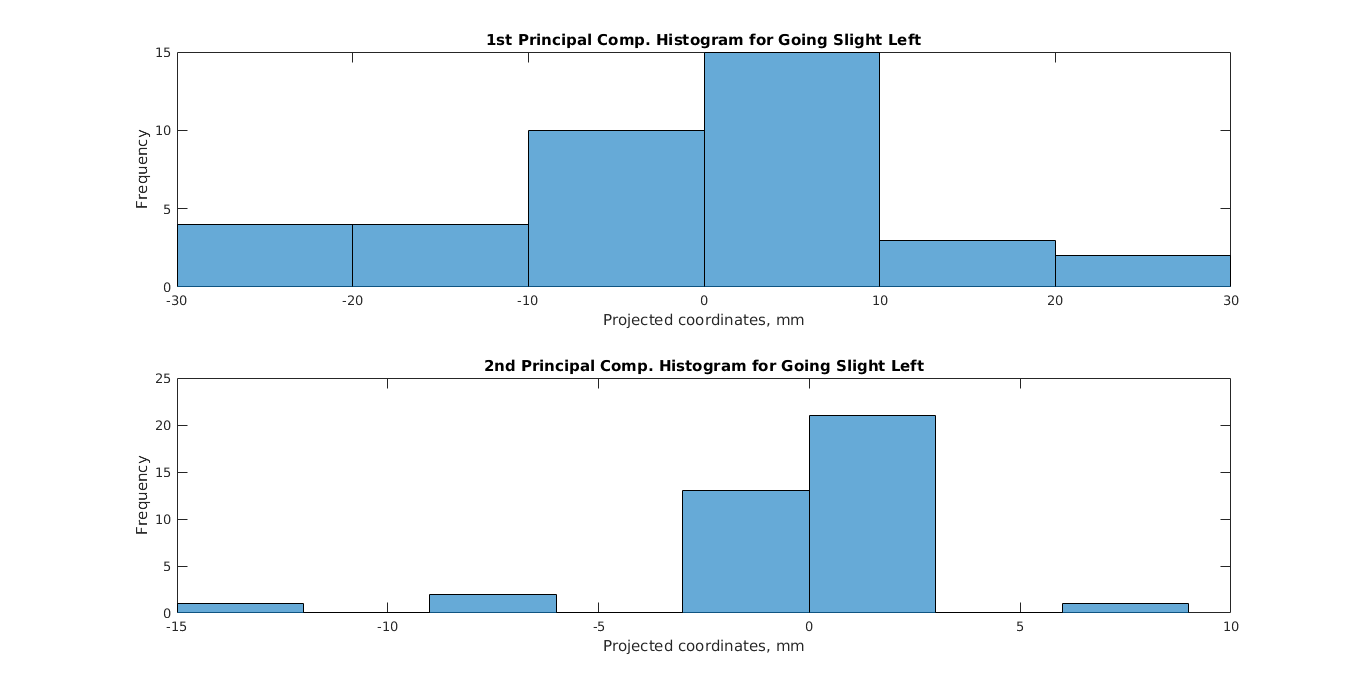
\includegraphics[width=\linewidth,fbox]{images/pca_histogram_slightLeft.png}
            \caption{Histograms of coordinates projected onto principal components for slight left movements.}
        \end{center}
    \end{figure}

    \newpage
    \subsection{Going slightly right}
    \begin{figure}[H]
        \begin{center}
            \setlength{\fboxsep}{0.5pt} %
            \setlength{\fboxrule}{0.5pt}
            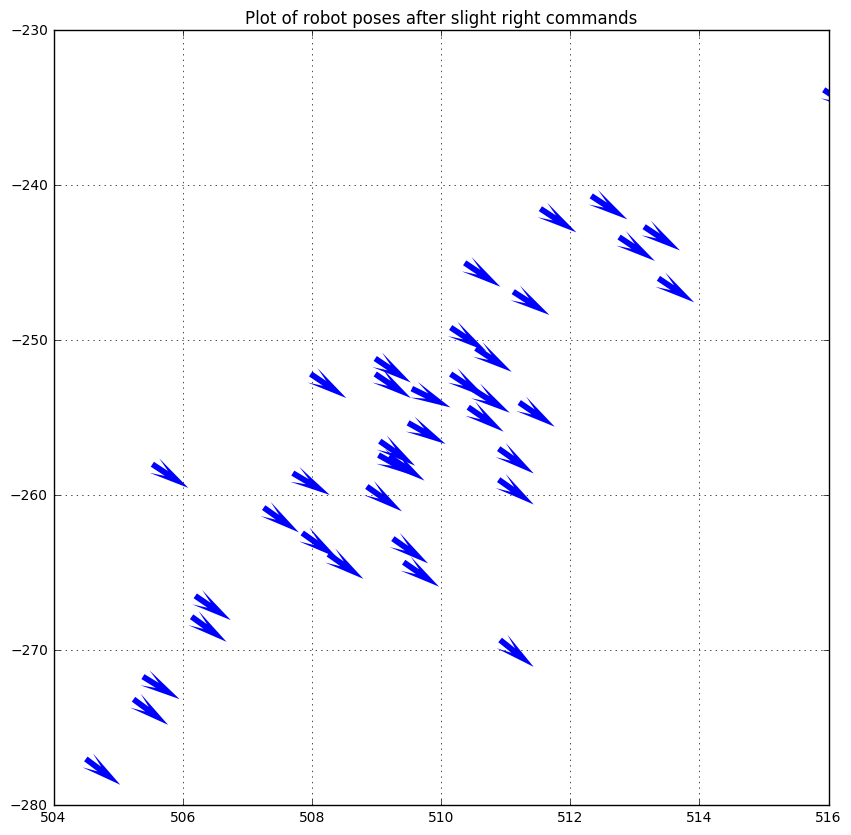
\includegraphics[width=12cm,fbox]{images/poses_plot_3_slightRight.png}
            \caption{Recorded poses of the LeJOS robot going slightly right.}
        \end{center}
    \end{figure}

    \begin{figure}[h!]
        \begin{center}
            \setlength{\fboxsep}{0.5pt} %
            \setlength{\fboxrule}{0.5pt}
            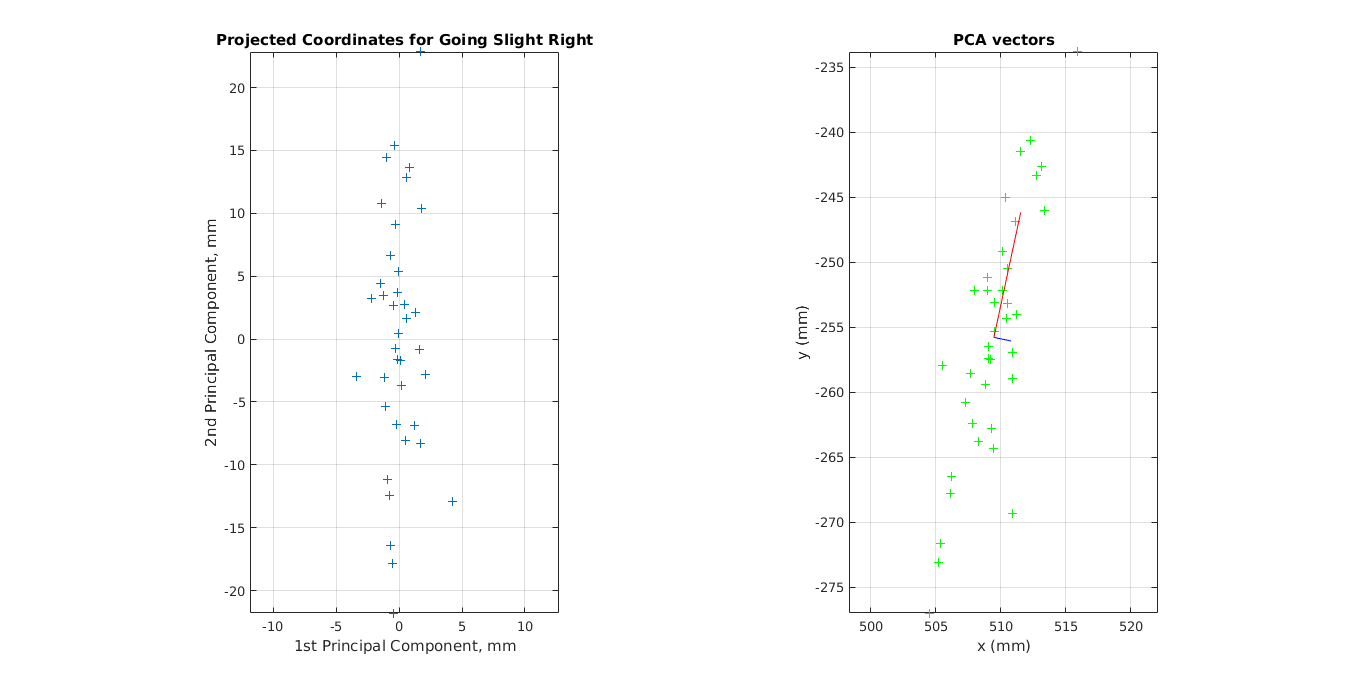
\includegraphics[width=\linewidth,fbox]{images/pca_slightRight.png}
            \caption{PCA analysis of slight right movements.}
        \end{center}
    \end{figure}

    \begin{figure}[h!]
        \begin{center}
            \setlength{\fboxsep}{0.5pt} %
            \setlength{\fboxrule}{0.5pt}
            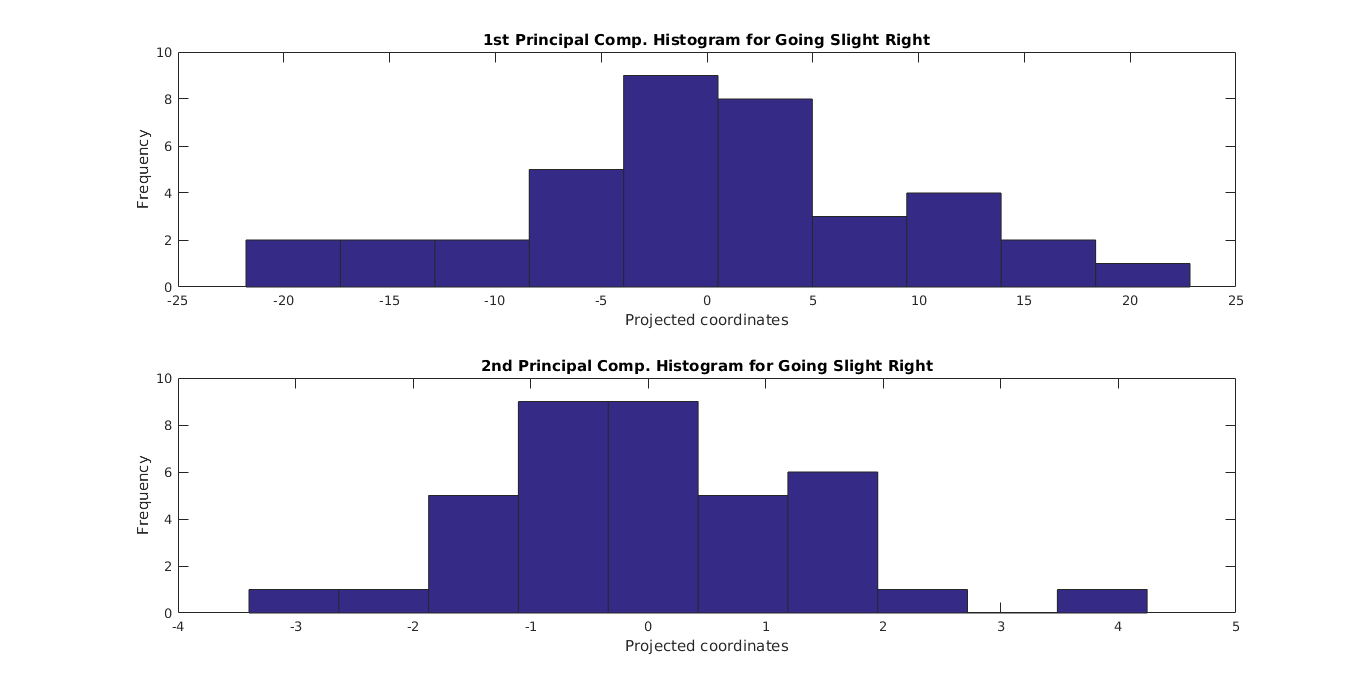
\includegraphics[width=\linewidth,fbox]{images/pca_histogram_slightRight.png}
            \caption{Histograms of coordinates projected onto principal components for slight right movements.}
        \end{center}
    \end{figure}

    \newpage
    \subsection{Going left}
    \begin{figure}[h!]
        \begin{center}
            \setlength{\fboxsep}{0.5pt} %
            \setlength{\fboxrule}{0.5pt}
            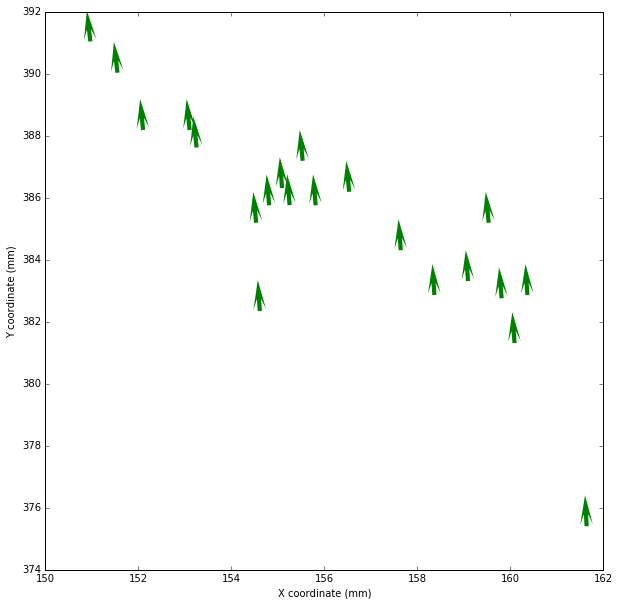
\includegraphics[width=12cm,fbox]{images/poses_plot_4_left.png}
            \caption{Recorded poses of the LeJOS robot going left.}
        \end{center}
    \end{figure}

    \begin{figure}[h!]
        \begin{center}
            \setlength{\fboxsep}{0.5pt} %
            \setlength{\fboxrule}{0.5pt}
            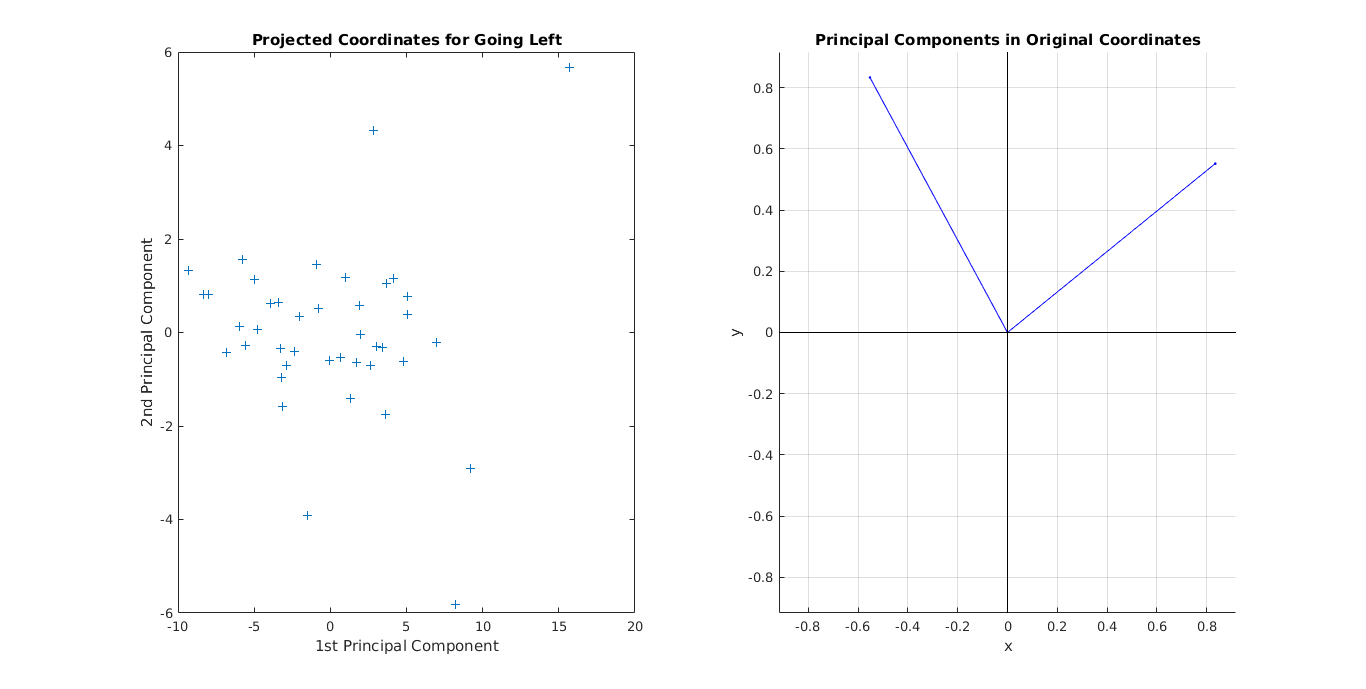
\includegraphics[width=\linewidth,fbox]{images/pca_Left.png}
            \caption{PCA analysis of hard left movements.}
        \end{center}
    \end{figure}
    
    \begin{figure}[h!]
        \begin{center}
            \setlength{\fboxsep}{0.5pt} %
            \setlength{\fboxrule}{0.5pt}
            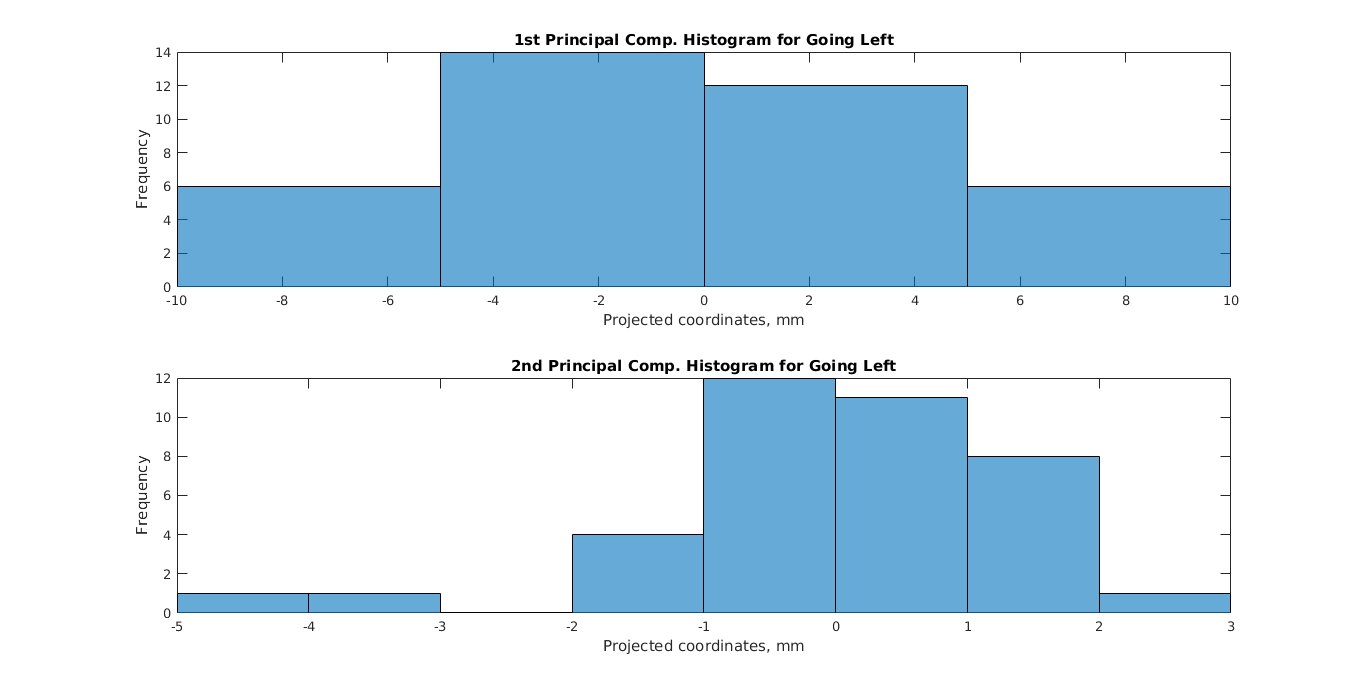
\includegraphics[width=\linewidth,fbox]{images/pca_histogram_Left.png}
            \caption{Histograms of coordinates projected onto principal components for hard left movements.}
        \end{center}
    \end{figure}

    \newpage
    \subsection{Going right}
    \begin{figure}[h!]
        \begin{center}
            \setlength{\fboxsep}{0.5pt} %
            \setlength{\fboxrule}{0.5pt}
            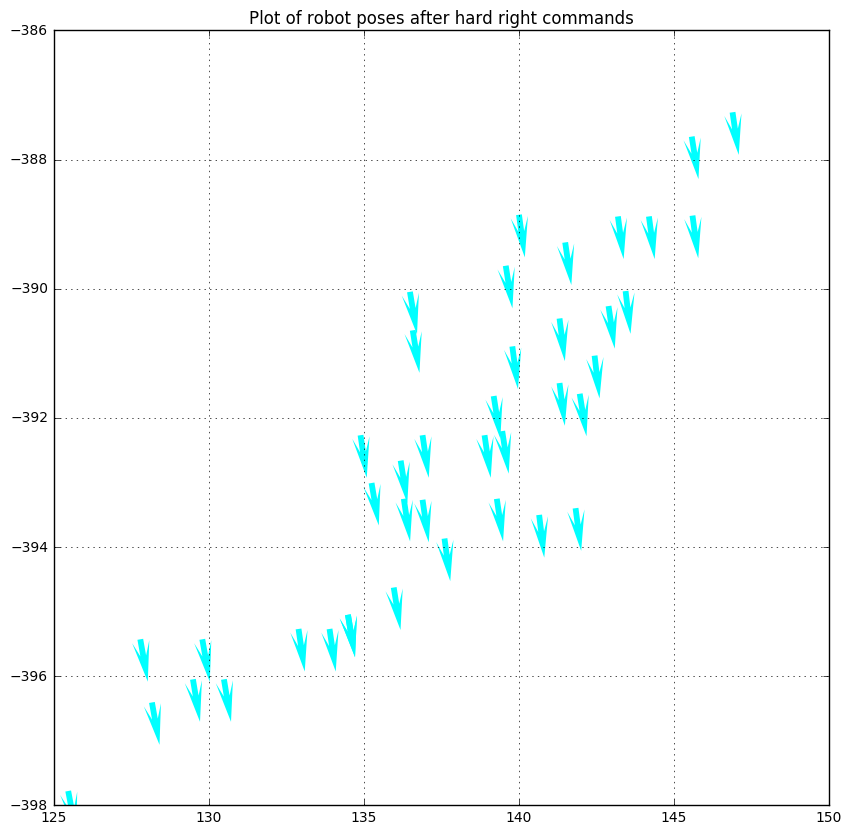
\includegraphics[width=12cm,fbox]{images/poses_plot_5_right.png}
            \caption{Recorded poses of the LeJOS robot going right.}
        \end{center}
    \end{figure}

    \begin{figure}[h!]
        \begin{center}
            \setlength{\fboxsep}{0.5pt} %
            \setlength{\fboxrule}{0.5pt}
            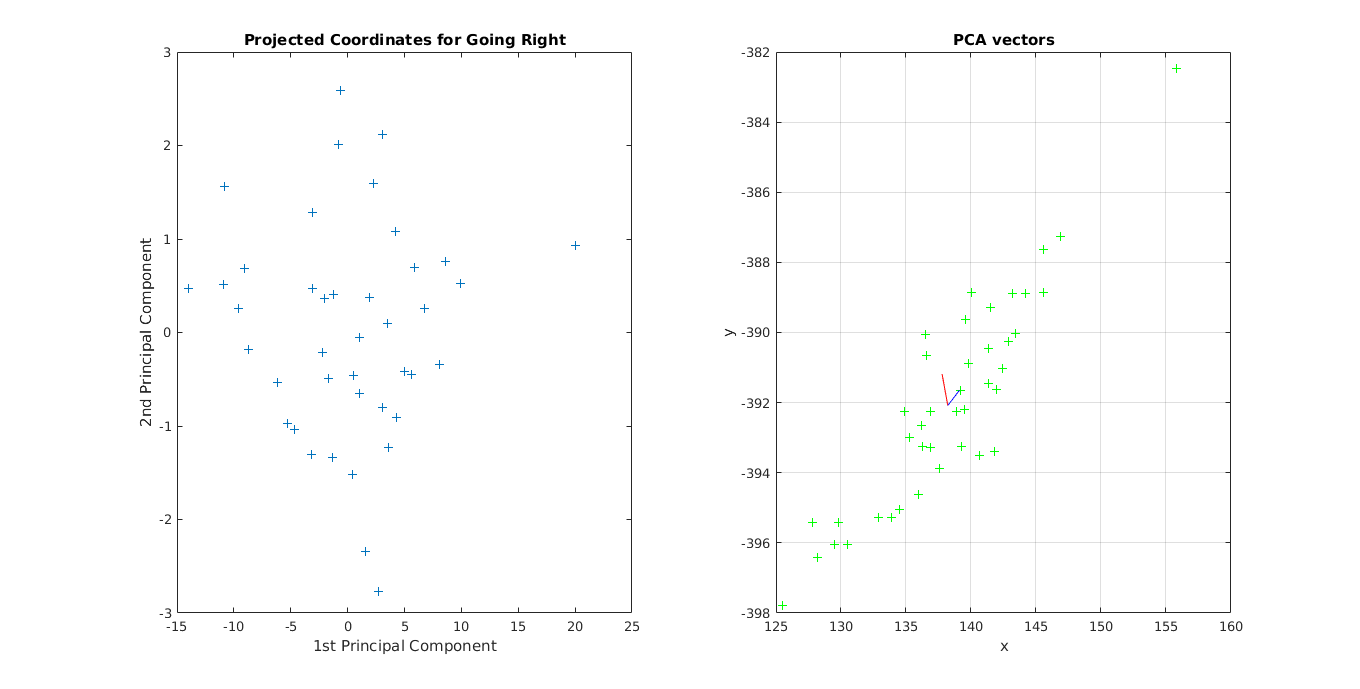
\includegraphics[width=\linewidth,fbox]{images/pca_Right.png}
            \caption{PCA analysis of hard right movements.}
        \end{center}
    \end{figure}
    
    \begin{figure}[h!]
        \begin{center}
            \setlength{\fboxsep}{0.5pt} %
            \setlength{\fboxrule}{0.5pt}
            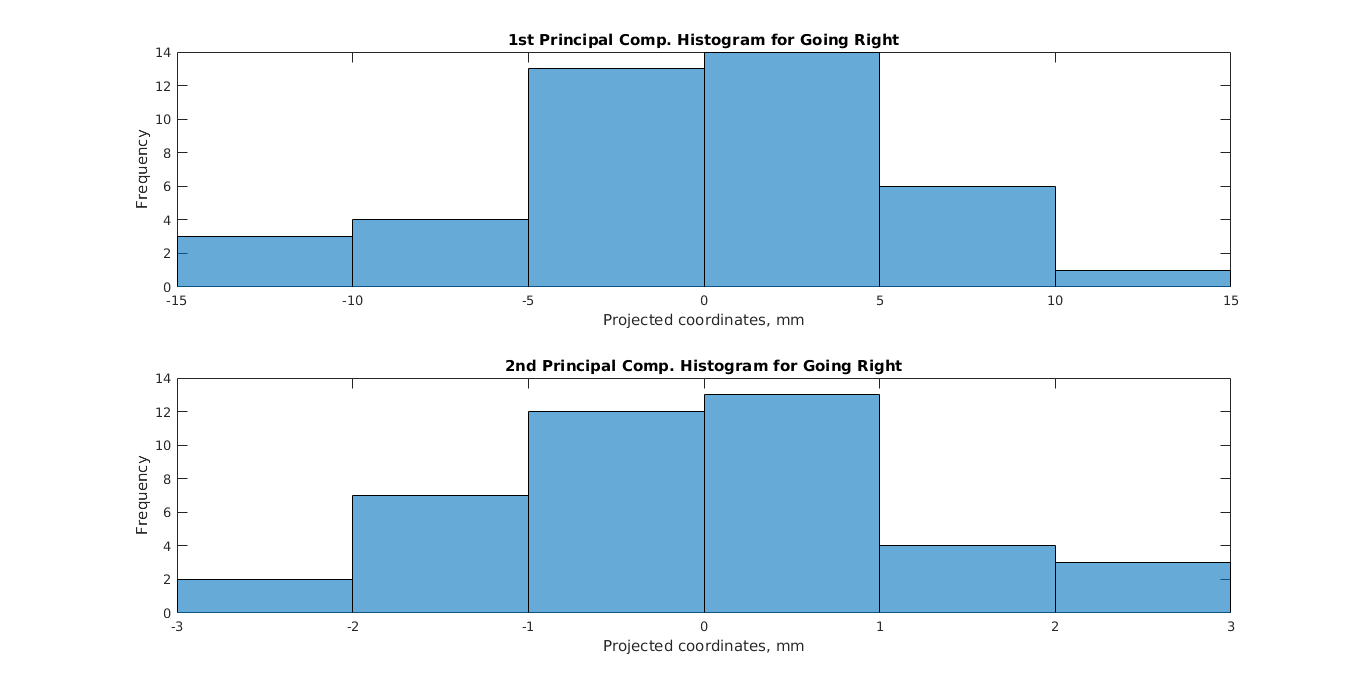
\includegraphics[width=\linewidth,fbox]{images/pca_histogram_Right.png}
            \caption{Histograms of coordinates projected onto principal components for hard right movements.}
        \end{center}
    \end{figure}

\end{document}
